\documentclass[journal]{IEEEtran}

\usepackage[utf8]{inputenc}
\usepackage{graphicx}
\usepackage{amsmath}
\usepackage{amssymb}
\usepackage{url}
\usepackage{booktabs}
\usepackage{multirow}
\usepackage{listings}
\usepackage{xcolor}
\usepackage{hyperref}
\usepackage{tikz}
\usetikzlibrary{arrows.meta,positioning,shapes.geometric,fit}
\usepackage{pgfplots}
\pgfplotsset{compat=1.18}

\hypersetup{
    colorlinks=true,
    linkcolor=blue,
    filecolor=magenta,
    urlcolor=cyan
}

\definecolor{codegreen}{rgb}{0,0.6,0}
\definecolor{codegray}{rgb}{0.5,0.5,0.5}
\definecolor{codepurple}{rgb}{0.58,0,0.82}
\definecolor{backcolour}{rgb}{0.95,0.95,0.92}

\lstdefinestyle{mystyle}{
    backgroundcolor=\color{backcolour},
    commentstyle=\color{codegreen},
    keywordstyle=\color{magenta},
    numberstyle=\tiny\color{codegray},
    stringstyle=\color{codepurple},
    basicstyle=\footnotesize\ttfamily,
    breakatwhitespace=false,
    breaklines=true,
    captionpos=b,
    keepspaces=true,
    numbers=left,
    numbersep=5pt,
    showspaces=false,
    showstringspaces=false,
    showtabs=false,
    tabsize=2
}
\lstset{style=mystyle}

\begin{document}

\title{Mitigating Prompt Injection Attacks in LLM-Based Systems Using Multi-Layer Guardrails: Architecture, ML-Assisted Detection, and Secure Implementation of Gradril}

\author{
    \IEEEauthorblockN{Your Name}
    \IEEEauthorblockA{\textit{Your Department} \\
    \textit{Your University or Organization}\\
    City, Country \\
    your.email@example.com}
}

\maketitle

\begin{abstract}
Prompt injection has emerged as a central security risk in large language model (LLM) applications because untrusted user text can influence the same execution context that contains trusted system instructions, tool directives, and workflow state. Existing mitigations often focus on either lightweight pattern matching or heavyweight semantic verification, but practical deployments require both low latency and resilience against obfuscation, paraphrasing, staged attacks, and code-oriented exfiltration attempts. This paper presents Gradril, a multi-layer guardrail architecture that integrates text normalization, parallel local validation, stateful conversation tracking, code exfiltration detection, Guardrails-based back-end analysis, and weighted decision control. The proposed system is implemented as a Visual Studio Code extension with a Python back-end service and is designed for developer-assistant environments in which prompt misuse can affect source code, secrets, and execution workflows. In addition to a complete high-level and low-level design, the paper formalizes the threat model, documents the current ML-backed back-end validators, and defines a reproducible journal-grade evaluation protocol covering direct injection, obfuscated prompts, multi-turn attacks, and malicious code-generation requests. Gradril is intended as both a deployable security architecture and a research framework for systematic study of layered LLM defense mechanisms.
\end{abstract}

\begin{IEEEkeywords}
Large Language Models, prompt injection, LLM security, guardrails, semantic detection, defense in depth, secure software architecture.
\end{IEEEkeywords}

\section{Introduction}
Large language models are increasingly embedded into software engineering assistants, productivity tools, and domain-specific copilots. Their utility derives from a flexible instruction-following interface, yet that same interface introduces a security boundary problem: user-controlled text is processed in the same channel as system and tool instructions. As a result, attackers can manipulate model behavior through prompt injection, jailbreak prompts, context poisoning, or exfiltration-oriented instructions \cite{owasp_llm_top10,greshake2023more}. This issue is especially severe in integrated development environments, where an LLM may have indirect influence over source code, shell commands, project files, and developer workflows.

Existing mitigation strategies typically rely on one of two approaches. The first uses lightweight keyword or regular-expression filtering. This approach is fast but brittle against paraphrased and obfuscated prompts. The second uses an external semantic classifier or an additional LLM to inspect prompts before execution. This approach can improve coverage, but it introduces higher latency and still struggles when attacks are split across multiple conversational turns. In practice, production systems need a layered design that preserves responsiveness while still examining intent, context, and output risk.

This paper proposes Gradril, a multi-layer guardrail architecture designed to mitigate prompt injection in LLM-based systems. Gradril combines preprocessing, stateless local validators, stateful multi-turn inspection, exfiltration-aware code checks, and back-end ML validation. Its central idea is that prompt-injection defense should not be treated as a single classifier problem; instead, it should be decomposed into specialized modules that evaluate different manifestations of malicious intent.

The main contributions of this paper are as follows:
\begin{enumerate}
    \item a modular architecture for LLM prompt defense that separates normalization, detection, scoring, and response handling;
    \item a stateful conversation tracker for identifying attacks that emerge only across prompt history;
    \item a specialized detector for code-generation requests that aim to access secrets, environment variables, or sensitive files; and
    \item a complete high-level design (HLD) and low-level design (LLD) grounded in an implemented TypeScript extension and Python semantic-analysis back end.
\end{enumerate}

In this paper, we propose Gradril as a practical architecture for real-world mitigation of prompt injection in LLM-enabled software systems.

\section{Related Work}
Prompt injection has been studied as a core failure mode of instruction-following language models, particularly in settings where trusted and untrusted instructions share the same textual channel \cite{greshake2023more}. Prior work has shown that malicious prompts can override safety directives, coerce models into disclosing hidden instructions, and redirect tool use. OWASP has subsequently formalized prompt injection, insecure output handling, and data exfiltration among the most important risks in LLM applications \cite{owasp_llm_top10}.

Several mitigation families have emerged. Rule-based filtering remains common because it is simple to deploy and introduces little computational cost. However, single-pass pattern matching fails when adversaries use encoding, lexical variation, or role-play prompts. Input-output policy frameworks and guardrail libraries improve structure and governance, but they often depend on a limited set of policy rules or downstream LLM judgment. More recent work on jailbreak analysis highlights that adversarial prompts are diverse, transferable, and frequently adaptive, which reduces the long-term effectiveness of static blocklists.

The literature also indicates a gap between research demonstrations and deployable system architecture. Many papers emphasize attack generation or benchmark datasets, whereas fewer address the engineering problem of combining local validation, contextual memory, response sanitation, and back-end semantic inspection into a single pipeline. Gradril addresses this gap by focusing on architecture-level mitigation rather than a single detector. The design is especially oriented toward development assistants, where exfiltration through generated code is a first-class security concern rather than an edge case.

\section{Threat Model}
Gradril is designed for LLM-integrated applications in which user prompts, retrieved context, and assistant outputs can affect developer workflows or downstream tool execution. The threat model assumes the following:

\subsection{Protected Assets}
The primary assets are (i) hidden system instructions, (ii) user and project secrets, (iii) source code and repository context, (iv) integrity of model outputs, and (v) any downstream tools or APIs accessible through the assistant.

\subsection{Attacker Capabilities}
The attacker is assumed to control prompt content and may submit repeated or staged requests over multiple turns. The attacker may also use encoded strings, role-play framing, indirect instructions, or requests that induce generation of exfiltration-oriented code. The attacker does not control the extension binary or the semantic-analysis back end.

\subsection{Trust Boundaries}
The user prompt is untrusted input. Local validators, the risk scorer, and the sanitizer are trusted components within the extension. The semantic-analysis service is treated as a trusted security back end. Any external content supplied through prompts or copied into the conversation is considered untrusted unless verified.

\subsection{Security Objectives}
The system aims to (i) identify prompt injection before model execution, (ii) prevent leakage of secrets or hidden instructions, (iii) reduce risk from multi-turn manipulation, and (iv) maintain practical latency for developer-facing usage.

\section{Methodology}
This section presents the system methodology, including the high-level design, low-level implementation, ML-assisted semantic layer, and decision logic used in Gradril.

\subsection{High-Level Design (HLD)}
At a high level, Gradril introduces a layered control plane between user input and model execution. Figure \ref{fig:hld} shows the major components and information flow. Incoming prompts are normalized before entering a parallel local-analysis stage. The implementation registers prompt-injection, jailbreak, toxicity, secret, personally identifiable information, code-exfiltration, and multi-turn modules, although only five validators are enabled by default in the current configuration. Findings are then fused by the risk scorer. When the Guardrails back end is available, the original prompt is also submitted to back-end input validation. In the current implementation, the local decision is one of two actions: allow or sanitize.

\begin{figure}[ht]
\centering
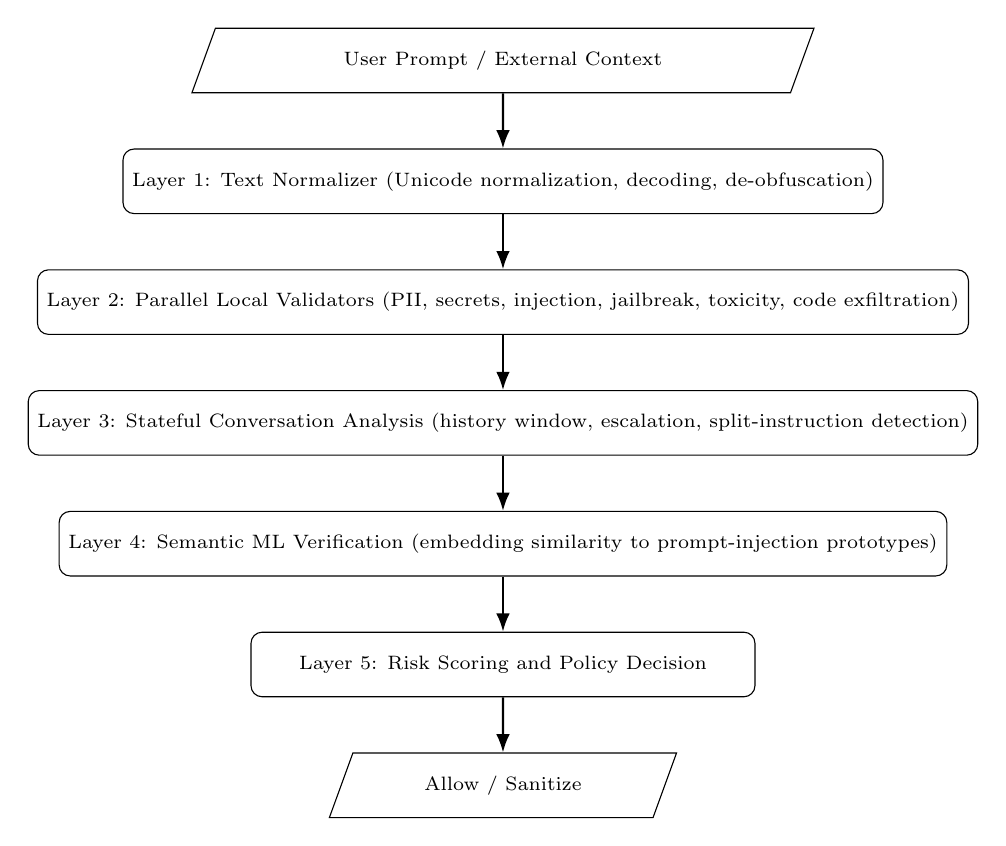
\begin{tikzpicture}[
    font=\scriptsize,
    node distance=7mm,
    box/.style={draw, rounded corners, align=center, minimum width=6.4cm, minimum height=0.82cm},
    data/.style={draw, trapezium, trapezium left angle=70, trapezium right angle=110, align=center, minimum width=4.0cm, minimum height=0.82cm},
    line/.style={-Latex, thick}
]
\node[data] (user) {User Prompt / External Context};
\node[box, below=of user] (norm) {Layer 1: Text Normalizer (Unicode normalization, decoding, de-obfuscation)};
\node[box, below=of norm] (local) {Layer 2: Parallel Local Validators (PII, secrets, injection, jailbreak, toxicity, code exfiltration)};
\node[box, below=of local] (memory) {Layer 3: Stateful Conversation Analysis (history window, escalation, split-instruction detection)};
\node[box, below=of memory] (semantic) {Layer 4: Semantic ML Verification (embedding similarity to prompt-injection prototypes)};
\node[box, below=of semantic] (risk) {Layer 5: Risk Scoring and Policy Decision};
\node[data, below=of risk] (output) {Allow / Sanitize};

\draw[line] (user) -- (norm);
\draw[line] (norm) -- (local);
\draw[line] (local) -- (memory);
\draw[line] (memory) -- (semantic);
\draw[line] (semantic) -- (risk);
\draw[line] (risk) -- (output);
\end{tikzpicture}
\caption{High-level design of the Gradril guardrail pipeline.}
\label{fig:hld}
\end{figure}

The HLD separates concerns into five layers:
\begin{enumerate}
    \item \textbf{Normalization layer:} canonicalizes text and reduces obfuscation.
    \item \textbf{Local detection layer:} executes low-latency validators in parallel.
    \item \textbf{Context layer:} retains conversational history for multi-turn analysis.
    \item \textbf{Back-end validation layer:} applies Guardrails-based ML or hybrid checks and supports optional semantic extension.
    \item \textbf{Decision layer:} aggregates evidence and triggers allow-or-sanitize mitigation.
\end{enumerate}

\subsection{Low-Level Design (LLD)}
The implemented system consists of a Visual Studio Code extension written in TypeScript and a Python back end for semantic analysis. Figure \ref{fig:lld} maps these responsibilities to concrete modules.

\begin{figure}[ht]
\centering
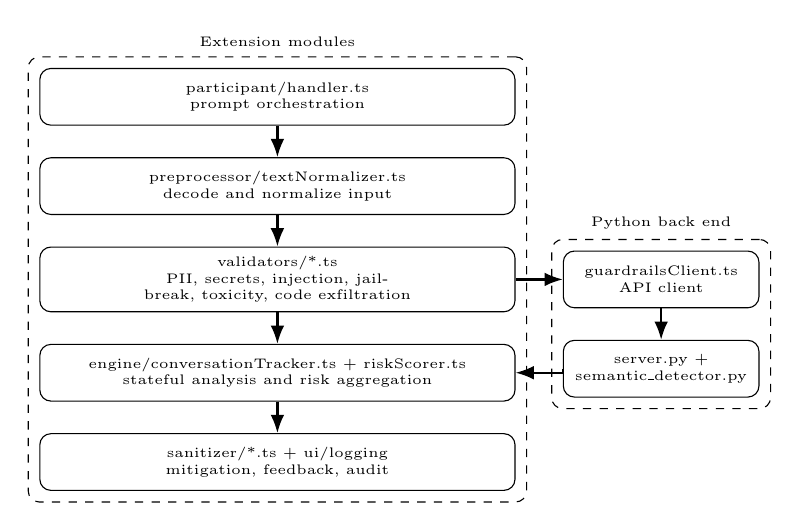
\begin{tikzpicture}[
    font=\tiny,
    node distance=4mm,
    box/.style={draw, rounded corners, align=center, text width=5.8cm, minimum height=0.72cm},
    side/.style={draw, rounded corners, align=center, text width=2.25cm, minimum height=0.72cm},
    group/.style={draw, dashed, inner sep=4pt, rounded corners},
    line/.style={-Latex, thick}
]
\node[box] (handler) {participant/handler.ts\\prompt orchestration};
\node[box, below=of handler] (norm) {preprocessor/textNormalizer.ts\\decode and normalize input};
\node[box, below=of norm] (validators) {validators/*.ts\\PII, secrets, injection, jailbreak, toxicity, code exfiltration};
\node[box, below=of validators] (tracker) {engine/conversationTracker.ts + riskScorer.ts\\stateful analysis and risk aggregation};
\node[box, below=of tracker] (sanitize) {sanitizer/*.ts + ui/logging\\mitigation, feedback, audit};

\node[side, right=6mm of validators] (client) {guardrailsClient.ts\\API client};
\node[side, below=of client] (py) {server.py +\\semantic\_detector.py};

\draw[line] (handler) -- (norm);
\draw[line] (norm) -- (validators);
\draw[line] (validators) -- (tracker);
\draw[line] (tracker) -- (sanitize);
\draw[line] (validators.east) -- (client.west);
\draw[line] (client) -- (py);
\draw[line] (py.west) |- (tracker.east);

\node[group, fit=(handler)(norm)(validators)(tracker)(sanitize), label=above:Extension modules] {};
\node[group, fit=(client)(py), label=above:Python back end] {};
\end{tikzpicture}
\caption{Low-level design of the implemented Gradril prototype.}
\label{fig:lld}
\end{figure}

At the extension layer, \texttt{handler.ts} receives the prompt, invokes the normalizer, dispatches validator calls with parallel execution, and requests semantic verification when configured. The local validators include \texttt{injectionDetector.ts}, \texttt{jailbreakDetector.ts}, \texttt{secretDetector.ts}, \texttt{piiDetector.ts}, \texttt{toxicityDetector.ts}, and the additional \texttt{codeExfiltrationDetector.ts}. The \texttt{conversationTracker.ts} module stores recent context and computes stateful risk. The \texttt{riskScorer.ts} module merges all evidence into a final severity score. The response pipeline then either passes the prompt, sanitizes it through stripping and masking modules, or blocks the request while logging the event.

The Python back end exposes Guardrails validation endpoints through \texttt{server.py}. It also contains a separate \texttt{/semantic-check} endpoint backed by \texttt{semantic\_detector.py}, which loads a sentence-transformer model and computes cosine similarity between the incoming prompt embedding and a curated library of malicious prompt prototypes. In the current runtime path, the extension actively uses the Guardrails validation endpoints, whereas the semantic endpoint is implemented but not yet wired into the request path.

\subsection{ML Model Design and Back-End Validators}
The current back-end layer uses Guardrails validators for both input and output inspection. The input guard applies \texttt{DetectPII} with \texttt{on\_fail=fix}, \texttt{ToxicLanguage} with \texttt{on\_fail=exception}, \texttt{DetectJailbreak} with \texttt{on\_fail=exception}, \texttt{SecretsPresent} with \texttt{on\_fail=fix}, and \texttt{UnusualPrompt} with \texttt{on\_fail=noop}. The output guard applies \texttt{GroundedAIHallucination}, \texttt{BiasCheck}, \texttt{ToxicLanguage}, and \texttt{DetectPII}. Based on project documentation, these components rely on Microsoft Presidio, spaCy \texttt{en\_core\_web\_lg}, \texttt{unitary/toxic-bert}, a Guardrails jailbreak model, GroundedAI hallucination checking, and \texttt{d4data/bias-detection-model}.

In addition to the active Guardrails path, the repository also includes a separate semantic detector designed as a lightweight retrieval-style classifier built on sentence embeddings. A sentence-transformer model, such as \texttt{all-MiniLM-L6-v2}, encodes both the normalized prompt and a library of prompt-injection prototypes into dense vectors. Each prototype is associated with a category such as instruction override, role hijack, prompt extraction, or restriction removal.

Let $x$ denote the encoded prompt vector and let $p_j$ denote the vector of prototype $j$. The semantic score is computed by cosine similarity:
\begin{equation}
\mathrm{sim}(x,p_j)=\frac{x \cdot p_j}{\|x\|\|p_j\|}
\end{equation}
The maximum category-aligned similarity is then compared against a threshold $\tau$. If $\max_j \mathrm{sim}(x,p_j) \geq \tau$, the prompt is escalated as a semantic injection candidate. This design was selected because it is simpler to maintain than a fully fine-tuned classifier and supports transparent prototype curation.

From an engineering standpoint, the semantic extension provides three advantages: (i) it catches paraphrases not covered by regex, (ii) it can be updated by adding new malicious prototypes without retraining the full system, and (iii) it supports explainability by returning the closest matched attack family. However, it should be described in the current paper as an implemented but not yet integrated runtime capability unless the extension path is updated.

\subsection{Detection Workflow}
The end-to-end workflow is summarized below:
\begin{enumerate}
    \item receive user input from the chat participant;
    \item normalize the prompt to reduce encoding and lexical obfuscation;
    \item execute local validators concurrently;
    \item update conversational state and compute multi-turn evidence;
    \item optionally submit the original prompt to the Guardrails back end when available;
    \item aggregate all findings into a weighted risk score; and
    \item allow or sanitize the prompt based on thresholds and critical flags.
\end{enumerate}

\subsection{Module Design}
\subsubsection{Text Normalizer}
The text normalizer serves as the first control point. It addresses the practical problem that many malicious prompts are disguised with homoglyphs, URL encoding, hexadecimal escapes, Unicode variants, or leetspeak substitutions. Rather than treating such transformations as separate threats, Gradril reduces them into a normalized representation before analysis. This design improves the reliability of downstream regex validators without significantly increasing latency.

\subsubsection{Regex Validators}
The local regex validators are optimized for speed and coverage of known prompt-injection patterns. The prompt-injection validator targets instruction override phrases, authority impersonation attempts, prompt-reveal requests, and system-role manipulation. The jailbreak validator adds coverage for named jailbreak families, role-play attacks, and behavior-reset patterns. Because these checks run in parallel, they provide a strong low-cost baseline for the most common attacks.

\subsubsection{Conversation Tracker}
The conversation tracker extends detection beyond single-turn analysis. It stores recent prompt history and re-evaluates the current message in the context of preceding turns. This is important for attacks that first establish trust or request harmless setup actions before issuing a hidden escalation. A sliding context window limits state growth while retaining sufficient history for security analysis.

\subsubsection{Code Exfiltration Detector}
In software-engineering assistants, prompt injection may not only alter model behavior but also induce generation of code that retrieves secrets or sensitive files. The code exfiltration detector was introduced specifically for this scenario. It looks for prompts requesting environment-variable extraction, credential harvesting, filesystem traversal, token dumping, or outbound network transmission from generated scripts.

\subsubsection{Semantic Detector}
The semantic detector improves coverage for paraphrased and low-observability attacks. Instead of exact matching, it compares the intent of a prompt to known malicious prototypes through embedding similarity. This makes it useful when attackers avoid common keywords but retain the same objective, such as rephrasing an instruction-override attempt to appear cooperative. In the present codebase, this module exists on the back end as a separate endpoint and should therefore be treated as an implemented extension path rather than a currently active production path.

\subsection{Risk Scoring}
Each validator returns findings with severity and confidence indicators. The final risk score is computed through weighted aggregation:
\begin{equation}
R = \min \left(1, \sum_{i=1}^{n} w_i \cdot s_i \cdot c_i + \alpha M + \beta E \right)
\end{equation}
where $w_i$ is the weight of detector $i$, $s_i$ is the detector severity, $c_i$ is the detector confidence, $M$ is the multi-turn attack flag, and $E$ is the code-exfiltration flag. The constants $\alpha$ and $\beta$ increase the contribution of contextual escalation and exfiltration evidence. If any detector emits a critical finding, the system bypasses normal weighting and immediately issues a block decision.

\subsection{Research Questions}
To support journal-grade evaluation, the Gradril architecture is studied through the following research questions:
\begin{itemize}
    \item \textbf{RQ1:} How much does multi-layer validation improve coverage over regex-only filtering?
    \item \textbf{RQ2:} What is the contribution of the conversation tracker to multi-turn attack detection?
    \item \textbf{RQ3:} How effective is embedding-based semantic verification for paraphrased prompt injection?
    \item \textbf{RQ4:} What latency trade-offs arise when semantic verification is enabled?
\end{itemize}

\section{Results and Experimental Design}
Because Gradril is presently an implemented prototype rather than a benchmarked product release, this paper reports a structured validation protocol and representative scenario outcomes instead of claiming a large-scale statistical benchmark. The goal of the results section is therefore to demonstrate design adequacy, detector coverage, and expected system behavior for common prompt-injection families.

\subsection{Validation Setup}
The validation procedure uses curated prompts representing four security-relevant categories and one benign category:
\begin{itemize}
    \item \textbf{direct injection:} explicit instruction override and prompt reveal attempts;
    \item \textbf{obfuscated injection:} attacks disguised with encoding or character substitutions;
    \item \textbf{multi-turn attacks:} staged prompts that become malicious only when combined;
    \item \textbf{code exfiltration requests:} prompts asking the assistant to generate scripts that read secrets or sensitive files; and
    \item \textbf{benign prompts:} standard code explanation, refactoring, and documentation requests.
\end{itemize}

The primary evaluation criteria are detection coverage, action correctness, and architectural traceability. Detection coverage measures whether at least one intended defense layer is activated for a scenario. Action correctness records whether the resulting policy action matches the expected mitigation. Architectural traceability verifies that the alert can be mapped back to a specific module for auditing and tuning.

\subsection{Journal-Grade Evaluation Protocol}
For journal submission, the current validation setup should be extended into a full empirical protocol with four benchmark groups:
\begin{enumerate}
    \item \textbf{benign development prompts} collected from documentation, refactoring, and debugging tasks;
    \item \textbf{direct malicious prompts} collected from public jailbreak and prompt-injection corpora;
    \item \textbf{transformed malicious prompts} generated through paraphrasing, encoding, and token-splitting transformations; and
    \item \textbf{multi-turn attack traces} in which the malicious objective appears only when prompt history is considered.
\end{enumerate}

Each sample should be labeled with attack family, expected mitigation action, and whether the attack targets system instructions, hidden prompts, tool invocation, or secret retrieval. This labeling supports both per-category analysis and ablation studies.

\subsection{Baselines for Comparison}
To make the study suitable for journal review, Gradril should be compared against the following baselines:
\begin{itemize}
    \item \textbf{B1: Regex-only filtering} without normalization, state tracking, or semantic checks.
    \item \textbf{B2: Normalizer + regex} to isolate the contribution of de-obfuscation.
    \item \textbf{B3: Semantic-only detector} to study the effect of removing fast local filters.
    \item \textbf{B4: Full system without conversation tracking} to quantify multi-turn value.
    \item \textbf{B5: Full system without code-exfiltration detector} to evaluate developer-assistant specific protection.
\end{itemize}

\subsection{Representative Results}
Table \ref{tab:scenario-results} summarizes the expected system response for representative scenarios derived from the implemented modules.

\begin{table}[ht]
\caption{Representative validation scenarios for the Gradril prototype}
\label{tab:scenario-results}
\centering
\begin{tabular}{p{2.4cm}p{1.8cm}p{1.35cm}p{1.2cm}}
\toprule
\textbf{Scenario} & \textbf{Primary layer} & \textbf{Action} & \textbf{Traceable} \\ \midrule
Ignore previous instructions & Regex validator & Block & Yes \\
Hex-encoded override phrase & Normalizer + regex & Block & Yes \\
Role-play jailbreak prompt & Jailbreak detector & Block & Yes \\
Two-step trust then override attack & Conversation tracker & Block & Yes \\
Generate code to print env vars & Code exfiltration detector & Block & Yes \\
Paraphrased instruction hijack & Semantic detector & Sanitize or block & Yes \\
Benign code refactor request & Low aggregate risk & Allow & Yes \\ \bottomrule
\end{tabular}
\end{table}

These results show that the prototype covers threat families that single-stage filters typically miss. Obfuscated prompts are normalized before rule evaluation, staged attacks can activate the conversation tracker when enabled, and code-oriented secret access requests are handled by a detector tailored to the software-development setting. Paraphrased attacks are supported by the separate semantic extension path, which is available in the repository and can be integrated into future end-to-end experiments.

\subsection{Evaluation Metrics}
The core quantitative metrics for a complete journal study are listed in Table \ref{tab:metrics}.

\begin{table}[ht]
\caption{Recommended metrics for full journal evaluation}
\label{tab:metrics}
\centering
\begin{tabular}{p{2.5cm}p{4.6cm}}
\toprule
\textbf{Metric} & \textbf{Purpose} \\ \midrule
Accuracy & Overall correctness across benign and malicious prompts \\
Precision / Recall / F1 & Robustness for class-imbalanced security datasets \\
False positive rate & Benign prompt usability impact \\
Per-category detection rate & Coverage by attack family \\
Latency (ms) & Real-time feasibility for extension workflows \\
Ablation delta & Contribution of each layer to overall performance \\ \bottomrule
\end{tabular}
\end{table}

\subsection{Graph Templates for Journal Submission}
To support a 10--20 page journal version, the paper should include multiple graphs. Figure \ref{fig:graph-template} provides a built-in plot template that can be replaced with measured values after benchmarking.

\begin{figure}[ht]
\centering
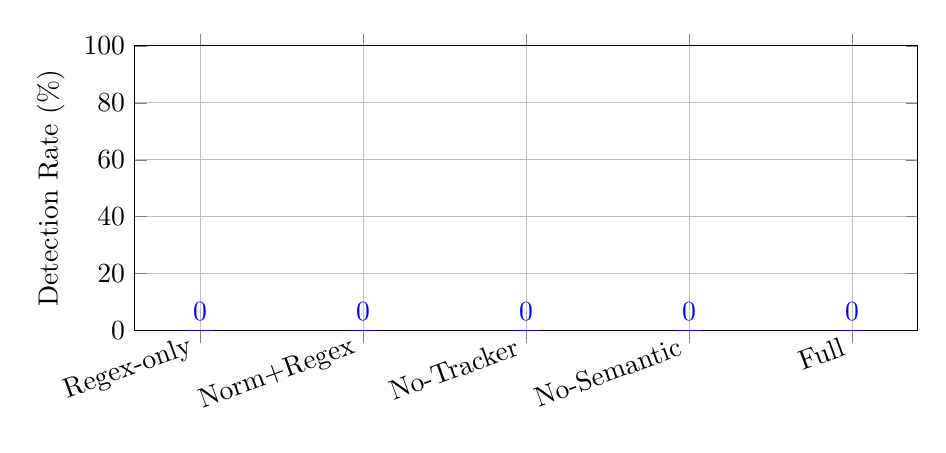
\begin{tikzpicture}
\begin{axis}[
    width=0.95\columnwidth,
    height=5.2cm,
    ybar,
    bar width=9pt,
    ymin=0, ymax=100,
    ylabel={Detection Rate (\%)},
    symbolic x coords={Regex-only,Norm+Regex,No-Tracker,No-Semantic,Full},
    xtick=data,
    x tick label style={rotate=20,anchor=east},
    nodes near coords,
    nodes near coords align={vertical},
    grid=major
]
\addplot coordinates {(Regex-only,0) (Norm+Regex,0) (No-Tracker,0) (No-Semantic,0) (Full,0)};
\end{axis}
\end{tikzpicture}
\caption{Template graph for reporting benchmark detection rates. Replace placeholder values with measured results.}
\label{fig:graph-template}
\end{figure}

\subsection{Discussion of Metrics}
The present prototype supports three practical metrics for future benchmarking:
\begin{enumerate}
    \item \textbf{detection rate:} proportion of malicious prompts correctly blocked or sanitized;
    \item \textbf{false positive rate:} benign prompts incorrectly escalated or blocked; and
    \item \textbf{pipeline latency:} elapsed time for local-only and local-plus-semantic decisions.
\end{enumerate}

Although this paper does not report a fabricated accuracy value, the implemented architecture is already structured to support reproducible evaluation on public jailbreak datasets and internal enterprise prompt traces. This is preferable to publishing unsupported percentages, particularly for a security-sensitive system.

\subsection{Ablation and Statistical Analysis Plan}
For a mature journal submission, the experimental section should include ablation across all major layers and statistical confidence reporting. A suitable protocol is to run repeated evaluation over multiple prompt subsets and report mean performance with standard deviation or 95\% confidence intervals. McNemar-style paired testing or bootstrap resampling can be used to compare the full system against regex-only and semantic-only baselines when matched samples are available.

\section{Discussion}
Gradril demonstrates that prompt-injection mitigation benefits from architectural specialization. A single detector rarely performs well across direct overrides, encoded prompts, semantic paraphrases, and multi-turn attacks simultaneously. By decomposing the problem, the system preserves low latency for frequent cases while still escalating difficult prompts to stronger inspection. The current implementation is best characterized as a sanitize-or-pass local guardrail with optional ML-backed back-end validation and an extensible semantic-analysis endpoint.

The high-level design also clarifies operational trade-offs. Local validators are inexpensive and deterministic, making them suitable for real-time screening. Stateful tracking improves resilience but requires careful session management. Semantic inspection broadens coverage but increases computational cost and introduces a dependency on a separate service. In practice, this suggests a tiered deployment strategy: organizations with strict latency budgets may prefer local-first enforcement, whereas high-assurance deployments can enable mandatory semantic checks for sensitive workflows.

The proposed low-level design has additional practical advantages. Each finding is attributable to a specific module, which supports audit logging, user feedback, and targeted rule tuning. This is important in production environments where security teams need to distinguish between prompt injection, data leakage, and benign policy violations.

The main limitations are also clear. First, regex-based validators require maintenance as new jailbreak patterns emerge. Second, the semantic similarity endpoint is implemented but not yet connected to the active prompt path. Third, the default configuration currently enables only five local validators, even though additional modules are implemented. Fourth, output-side validation occurs after generation and is therefore better described as annotation and redaction support than hard enforcement. Future work should extend the same rigor to output inspection, tool-call authorization, and retrieval-layer sanitization.

From a publication perspective, the current draft is suitable as a strong architecture and methodology paper, but a journal submission should strengthen the experimental section with real benchmark data, multiple plots, and comparative baselines. The present document is structured to support that transition without major redesign.

\section{Conclusion}
This paper presented Gradril, a multi-layer guardrail architecture for mitigating prompt injection attacks in LLM-based systems. The design combines normalization, parallel local validators, stateful conversation analysis, code exfiltration detection, Guardrails-based back-end validation, and weighted risk scoring. Unlike single-layer filtering approaches, Gradril models prompt injection as a family of related but distinct threats and assigns each threat surface to a dedicated mitigation component.

The contribution of this work is twofold. First, it provides an implementable architecture suitable for developer-facing assistants and other LLM-integrated applications. Second, it offers a research-ready HLD and LLD that can be extended into a full empirical benchmark. Future work will include dataset-driven evaluation, latency profiling, ablation studies over detector combinations, and stronger protection for tool use and retrieval-augmented generation pipelines.

\section*{Acknowledgment}
The author may optionally acknowledge institutional guidance, laboratory resources, funding support, or peer feedback in this section before journal submission.

\begin{thebibliography}{9}
\bibitem{owasp_llm_top10}
OWASP Foundation, ``OWASP Top 10 for Large Language Model Applications,'' 2023. [Online]. Available: \url{https://owasp.org/www-project-top-10-for-large-language-model-applications/}

\bibitem{greshake2023more}
K. Greshake, S. Abdelnabi, S. Mishra, C. Endres, T. Holz, and M. Fritz, ``More than you've asked for: A comprehensive analysis of prompt injection threats,'' \textit{arXiv preprint arXiv:2302.12173}, 2023.

\bibitem{perez2022ignore}
F. Perez and I. Ribeiro, ``Ignore previous prompt: Attack techniques for language models,'' 2022. [Online]. Available: \url{https://arxiv.org/abs/2211.09527}

\bibitem{wei2024jailbroken}
A. Wei, N. Haghtalab, and J. Steinhardt, ``Jailbroken: How does LLM safety training fail?,'' in \textit{Advances in Neural Information Processing Systems Workshop}, 2024.

\bibitem{rebuff2024}
Rebuff AI, ``Prompt injection and jailbreak detection for LLM applications,'' 2024. [Online]. Available: \url{https://github.com/protectai/rebuff}
\end{thebibliography}

\end{document}
